\documentclass[aspectratio=169, 10pt]{beamer}

\usepackage[utf8]{inputenc}
\usepackage[T1]{fontenc}
\usepackage[spanish, es-nodecimaldot]{babel}
\usepackage{amsmath, amssymb}
\usepackage{booktabs}
\usepackage{graphicx}
\usepackage{listings}
\usepackage{tikz}
\usetikzlibrary{arrows.meta, positioning, shapes.geometric}

% Aerospace color palette
\definecolor{AeroNavy}{RGB}{22, 54, 93}
\definecolor{AeroBlue}{RGB}{43, 92, 143}
\definecolor{AeroAccent}{RGB}{217, 95, 2}
\definecolor{AeroGreen}{RGB}{27, 158, 119}
\definecolor{CodeBg}{RGB}{246, 248, 250}

\usetheme{Madrid}
\usecolortheme{default}
\setbeamercolor{structure}{fg=AeroNavy}
\setbeamercolor{palette primary}{bg=AeroNavy, fg=white}
\setbeamercolor{palette secondary}{bg=AeroBlue, fg=white}
\setbeamercolor{palette tertiary}{bg=AeroNavy, fg=white}
\setbeamercolor{frametitle}{bg=AeroNavy, fg=white}
\setbeamercolor{block title}{bg=AeroBlue, fg=white}
\setbeamercolor{block body}{bg=AeroNavy!5, fg=black}

\setbeamertemplate{navigation symbols}{}
\setbeamertemplate{itemize items}[circle]

\lstset{
    language=Python,
    backgroundcolor=\color{CodeBg},
    basicstyle=\ttfamily\scriptsize,
    keywordstyle=\color{AeroBlue}\bfseries,
    commentstyle=\color{AeroGreen}\itshape,
    stringstyle=\color{AeroAccent},
    frame=single,
    rulecolor=\color{AeroBlue!40},
    showstringspaces=false,
    breaklines=true
}

\title[Misión ÍCARO · PEI2]{Misión ÍCARO: Análisis de Trayectoria Balística con Resistencia Aerodinámica}
\subtitle{Ejercicio 1 · Métodos Numéricos, Modelado Físico y GUI Interactiva en Python}
\author[ETSIAE · Programación]{Grado en Ingeniería Aeroespacial · ETSIAE}
\date{Curso 2026}

\begin{document}

% ============================================================================
% SLIDE 1: PORTADA
% ============================================================================
\begin{frame}[plain]
    \titlepage
    \begin{center}
        \vspace{-0.4cm}
        \small \textcolor{AeroBlue}{\textbf{Librerías científicas:} \texttt{numpy} $\cdot$ \texttt{scipy} $\cdot$ \texttt{matplotlib.widgets}}
    \end{center}
\end{frame}

% ============================================================================
% SLIDE 2: CONTEXTO FISICO E HILO CONDUCTOR
% ============================================================================
\begin{frame}{Contexto Físico e Hilo Conductor de la Misión}
    \textbf{Objetivo:} Procesar datos experimentales y de telemetría radar de una sonda atmosférica con freno aerodinámico pasivo mediante un flujo científico integral.

    \vspace{0.5cm}
    \begin{center}
    \begin{tikzpicture}[
        node distance=0.45cm,
        box/.style={rectangle, rounded corners=4pt, draw=AeroNavy, fill=AeroNavy!8,
                    thick, text width=3.55cm, align=center, minimum height=1.35cm, font=\scriptsize},
        arr/.style={-{Stealth[length=2.5mm]}, thick, color=AeroAccent}
    ]
        \node[box] (s1) {\textbf{1. Calibración}\\Sistema lineal $M\vec{a}=\vec{V}$\\$\vec{a}_0$ en plataforma};
        \node[box, right=of s1] (s2) {\textbf{2. Túnel de Viento}\\Regresión lineal\\Parámetro $(C_D A)$};
        \node[box, right=of s2] (s3) {\textbf{3. Atmósfera ISA}\\Interpolación 1D\\Densidad $\rho(405\,\mathrm{m})$};

        \node[box, below=0.8cm of s3] (s4) {\textbf{4. Cinemática Radar}\\Diferencias finitas\\Velocidad $v(t)$};
        \node[box, left=of s4] (s5) {\textbf{5. Energía Disipada}\\Integración numérica\\Trabajo $W_{\text{drag}}$};
        \node[box, left=of s5] (s6) {\textbf{6. Impacto Final}\\Búsqueda de raíces\\Instante $t_{\text{impacto}}$};

        \draw[arr] (s1) -- (s2);
        \draw[arr] (s2) -- (s3);
        \draw[arr] (s3) -- (s4);
        \draw[arr] (s4) -- (s5);
        \draw[arr] (s5) -- (s6);
    \end{tikzpicture}
    \end{center}

    \vspace{0.25cm}
    \begin{block}{Integración y Validación}
        Cada magnitud física se valida en \textbf{unidades SI}, se visualiza en una \textbf{GUI interactiva única} y se verifica con \textbf{tests unitarios funcionales}.
    \end{block}
\end{frame}

% ============================================================================
% SLIDE 3: ARQUITECTURA MODULAR Y CALIDAD DE CODIGO
% ============================================================================
\begin{frame}{Arquitectura Modular y Calidad del Código}
    \begin{columns}[T]
        \begin{column}{0.52\textwidth}
            \textbf{Separación estricta de responsabilidades:}
            \vspace{0.15cm}
            \begin{itemize}
                \item \texttt{my\_math.py}: Métodos numéricos puros (\texttt{numpy} / \texttt{scipy}).
                \item \texttt{physics.py}: Datos brutos, modelo físico e informe SI.
                \item \texttt{gui.py}: Interfaz gráfica exclusiva con \texttt{matplotlib}.
                \item \texttt{main.py}: Punto de entrada único del proyecto.
                \item \texttt{test\_math.py} y \texttt{test\_physics.py}: Tests unitarios funcionales.
            \end{itemize}
        \end{column}
        \begin{column}{0.45\textwidth}
            \begin{block}{Buenas Prácticas (Rúbrica)}
                \begin{itemize}
                    \item \textbf{Paradigma funcional:} Funciones \texttt{def} modulares, sin clases innecesarias.
                    \item \textbf{Vectorización:} Cero bucles \texttt{for} sobre arrays NumPy.
                    \item \textbf{Importaciones limpias:} \texttt{from numpy import ...} (sin alias \texttt{np}).
                    \item \textbf{Nomenclatura:} \texttt{snake\_case} descriptivo y docstrings en inglés.
                \end{itemize}
            \end{block}
        \end{column}
    \end{columns}
\end{frame}

% ============================================================================
% SLIDE 4: APARTADO 1 - CALIBRACION ACELEROMETRO
% ============================================================================
\begin{frame}{Apartado 1: Calibración de Plataforma (Sistema Lineal)}
    \begin{columns}[c]
        \begin{column}{0.43\textwidth}
            \textbf{Modelo Matemático:}
            \[
                M_{\text{calib}} \cdot \vec{a} = \vec{V}_{\text{medido}}
            \]
            \begin{itemize}
                \item Método: \texttt{scipy.linalg.solve} (factorización LU).
                \item $\vec{a} = [15.5426,\ -7.7063,\ 96.5568]\ \mathrm{m/s^2}$.
                \item $|\vec{a}| = 98.1028\ \mathrm{m/s^2}$ ($\approx 10.00\,g$).
            \end{itemize}

            \vspace{0.2cm}
            \begin{block}{Interpretación Física}
                $M_{\text{calib}}$ es diagonalmente dominante: fuerte impulso vertical en $Z$ y aceleraciones parásitas laterales pequeñas.
            \end{block}
        \end{column}
        \begin{column}{0.55\textwidth}
            \centering
            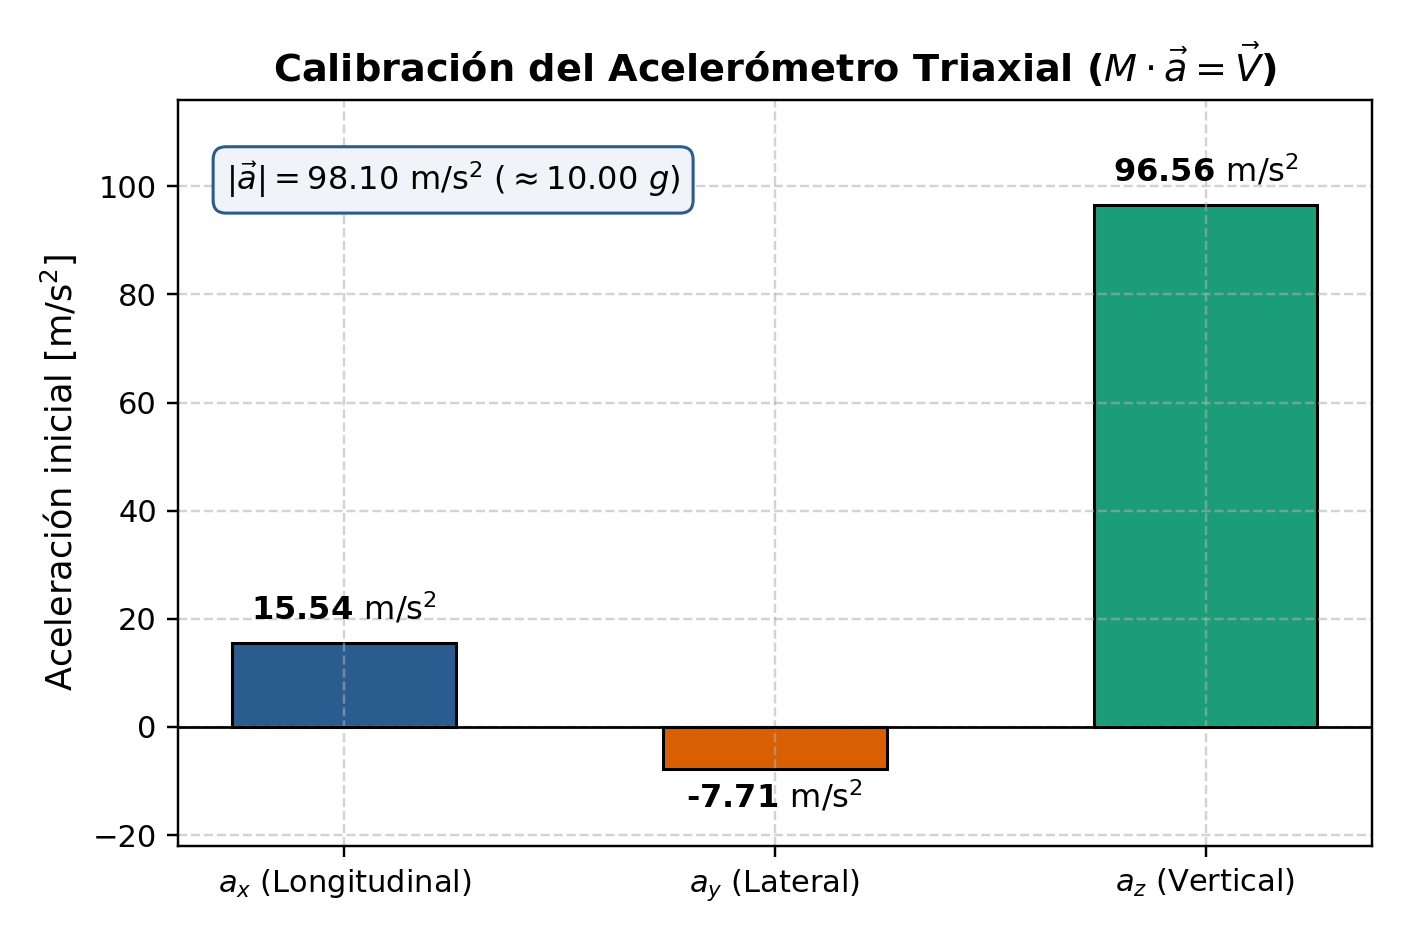
\includegraphics[width=\textwidth]{figures/fig_sec1.png}
        \end{column}
    \end{columns}
\end{frame}

% ============================================================================
% SLIDE 5: APARTADO 2 - REGRESION LINEAL TUNEL DE VIENTO
% ============================================================================
\begin{frame}{Apartado 2: Caracterización Aerodinámica (Regresión Lineal)}
    \begin{columns}[c]
        \begin{column}{0.43\textwidth}
            \textbf{Modelo Aerodinámico Subsónico:}
            \[
                F_D = (C_D A) \cdot q, \qquad q = \frac{1}{2}\rho v^2
            \]
            \begin{itemize}
                \item Mínimos cuadrados proporcionales y \texttt{numpy.polyfit}.
                \item $(C_D A) = 0.025270\ \mathrm{m^2}$.
                \item Bondad del ajuste: $R^2 = 0.999664$.
            \end{itemize}

            \vspace{0.2cm}
            \begin{block}{Orden de Magnitud}
                Para $q = 1000\ \mathrm{Pa}$, $F_D \approx 25.3\ \mathrm{N} \Rightarrow C_D A \approx 0.025\ \mathrm{m^2}$ (sonda compacta con freno pasivo).
            \end{block}
        \end{column}
        \begin{column}{0.55\textwidth}
            \centering
            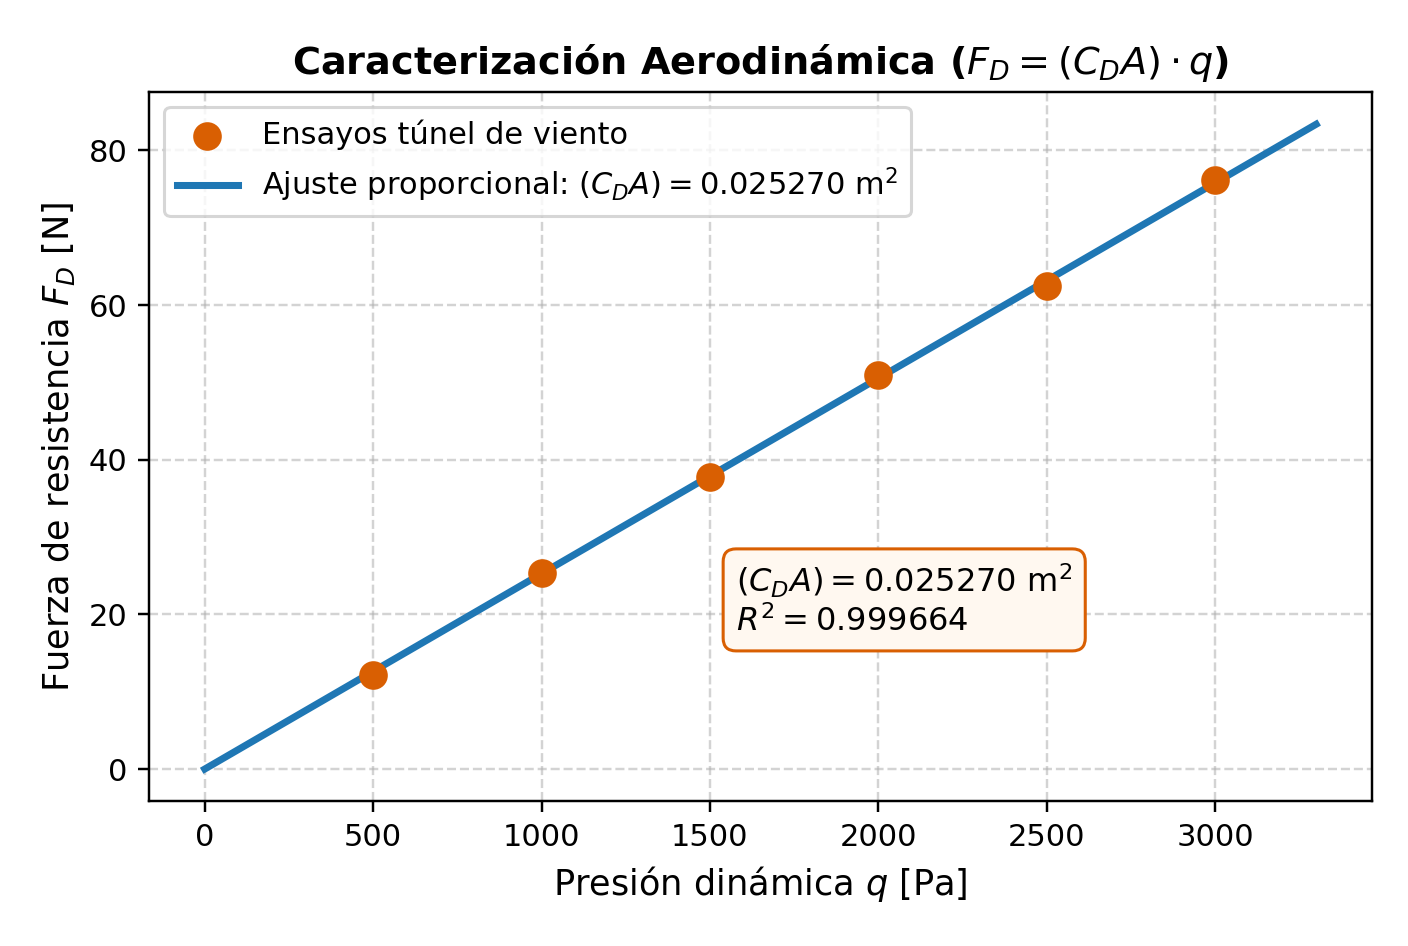
\includegraphics[width=\textwidth]{figures/fig_sec2.png}
        \end{column}
    \end{columns}
\end{frame}

% ============================================================================
% SLIDE 6: APARTADO 3 - INTERPOLACION ATMOSFERA ISA
% ============================================================================
\begin{frame}{Apartado 3: Modelo Atmosférico Local ISA (Interpolación 1D)}
    \begin{columns}[c]
        \begin{column}{0.43\textwidth}
            \textbf{Consulta en Apogeo ($h = 405\ \mathrm{m}$):}
            \begin{itemize}
                \item Método: \texttt{scipy.interpolate.interp1d} (\texttt{cubic} y \texttt{linear}).
                \item $\rho_{\text{cúbica}}(405\,\mathrm{m}) = 1.177687\ \mathrm{kg/m^3}$.
                \item $\rho_{\text{lineal}}(405\,\mathrm{m}) = 1.178020\ \mathrm{kg/m^3}$.
            \end{itemize}

            \vspace{0.2cm}
            \begin{block}{Interpretación Física}
                Entre $0\ \mathrm{m}$ ($1.225\ \mathrm{kg/m^3}$) y $500\ \mathrm{m}$ ($1.167\ \mathrm{kg/m^3}$), la densidad cae un $3.86\%$ acorde con la troposfera ISA.
            \end{block}
        \end{column}
        \begin{column}{0.55\textwidth}
            \centering
            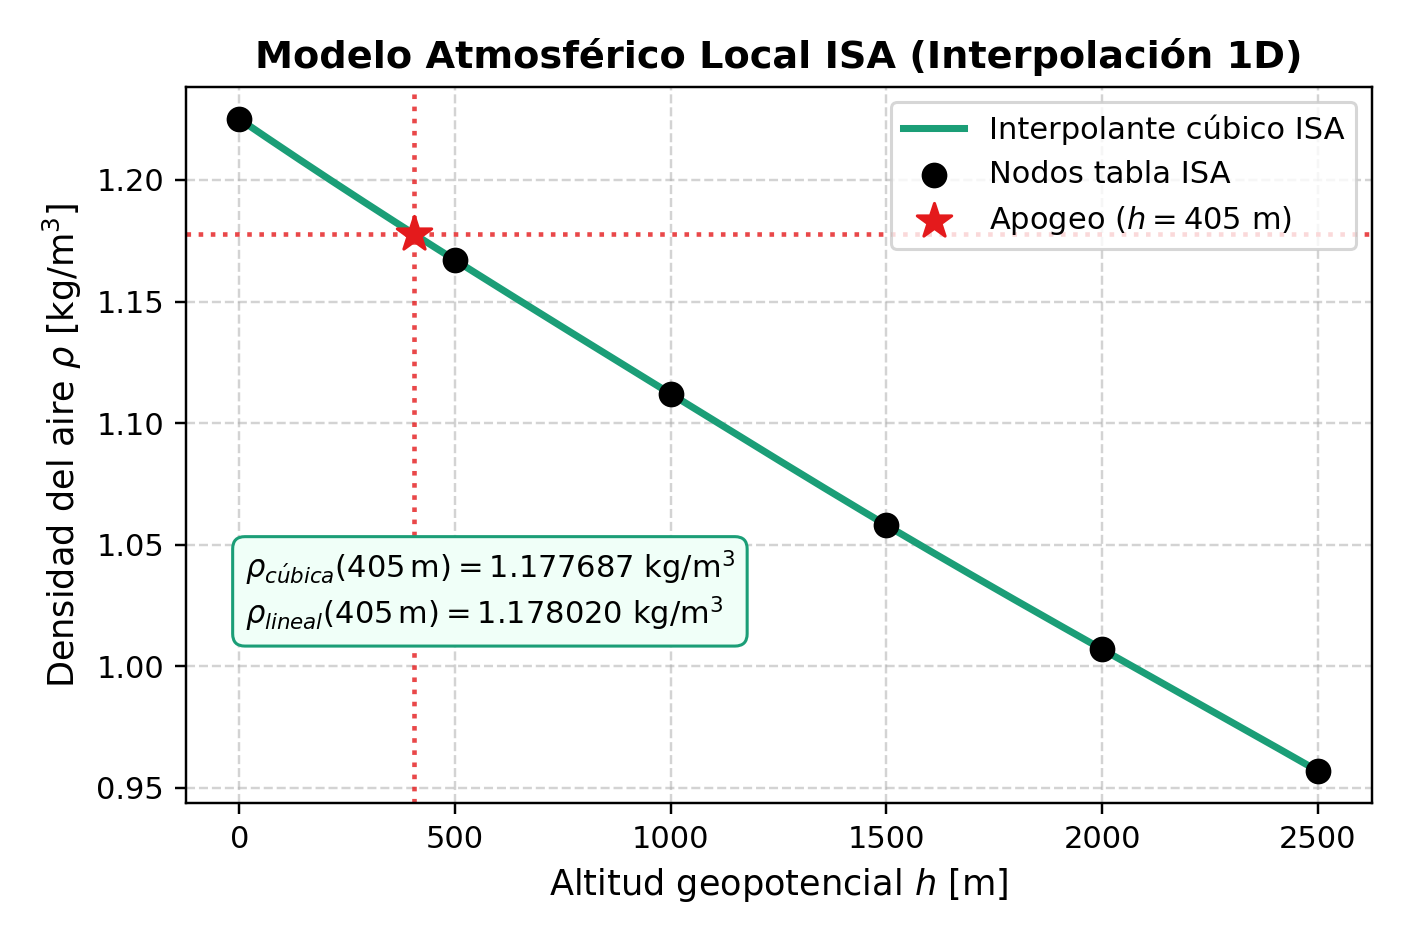
\includegraphics[width=\textwidth]{figures/fig_sec3.png}
        \end{column}
    \end{columns}
\end{frame}

% ============================================================================
% SLIDE 7: APARTADO 4 - DERIVACION NUMERICA VECTORIZADA
% ============================================================================
\begin{frame}[fragile]{Apartado 4: Cinemática del Vuelo (Diferencias Finitas)}
    \begin{columns}[c]
        \begin{column}{0.51\textwidth}
\begin{lstlisting}[basicstyle=\ttfamily\fontsize{5.5}{6.8}\selectfont]
def finite_difference_derivative(t_nodes, y_nodes):
    dt = t_nodes[1] - t_nodes[0]
    dy_dt = zeros_like(y_nodes, dtype=float)
    dy_dt[0] = (y_nodes[1] - y_nodes[0]) / dt
    dy_dt[1:-1] = (y_nodes[2:] - y_nodes[:-2]) / (2.0 * dt)
    dy_dt[-1] = (y_nodes[-1] - y_nodes[-2]) / dt
    return dy_dt
\end{lstlisting}
            \begin{itemize}
                \item Sin bucles \texttt{for}; sin errores de índice en extremos.
                \item $v(0) = 195.23\ \mathrm{m/s}$ (régimen subsónico).
                \item En apogeo ($t=4.5\ \mathrm{s}$): $v_y = 0\ \mathrm{m/s}$, $v = 63.25\ \mathrm{m/s}$.
            \end{itemize}
        \end{column}
        \begin{column}{0.47\textwidth}
            \centering
            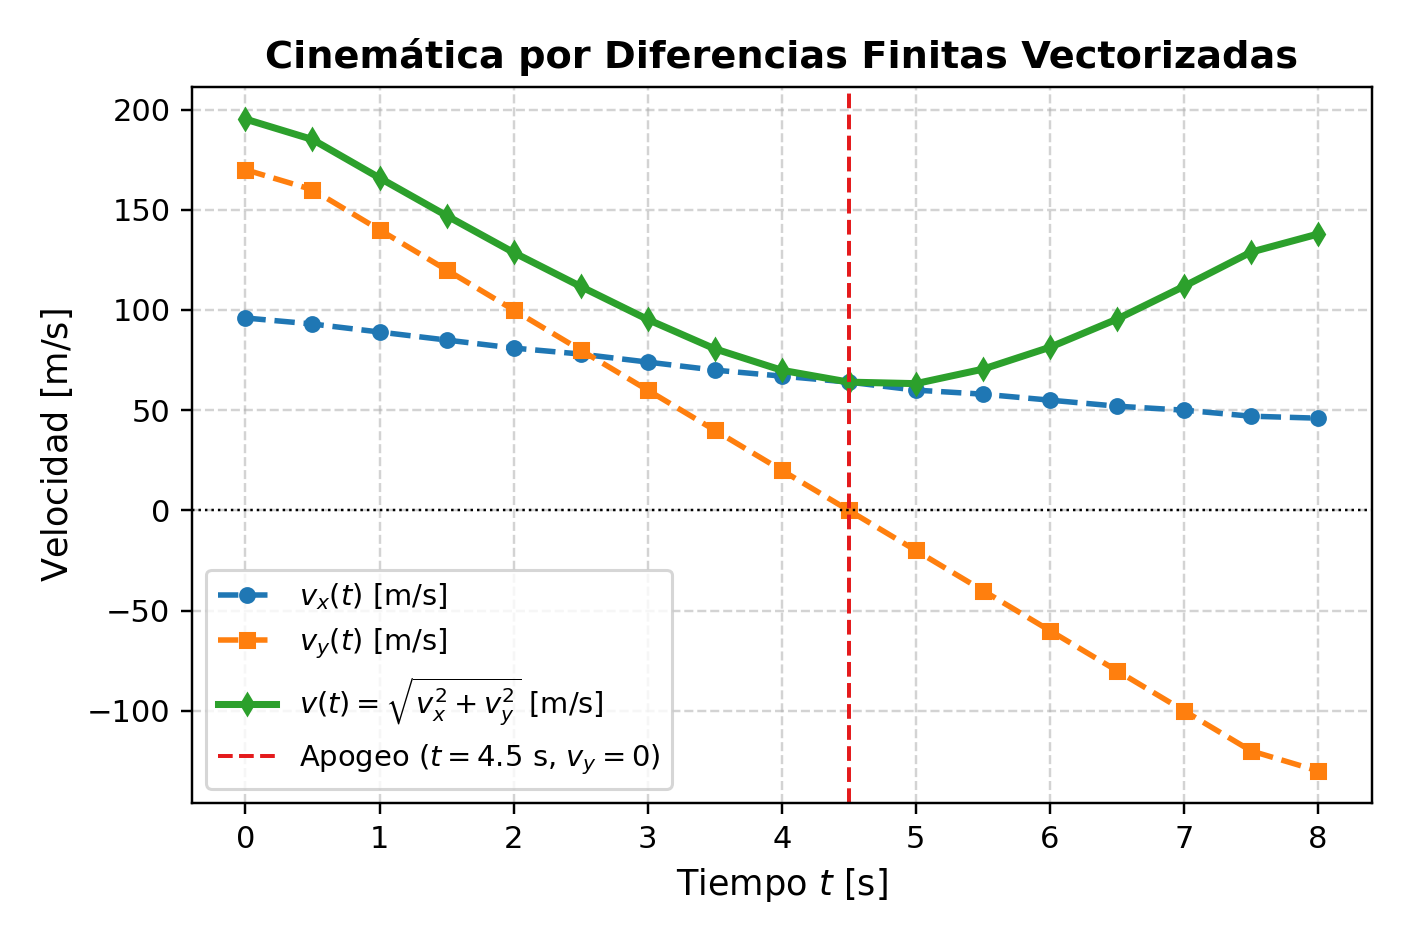
\includegraphics[width=\textwidth]{figures/fig_sec4.png}
        \end{column}
    \end{columns}
\end{frame}

% ============================================================================
% SLIDE 8: APARTADO 5 - INTEGRACION NUMERICA
% ============================================================================
\begin{frame}{Apartado 5: Energía Disipada por la Atmósfera (Integración)}
    \begin{columns}[c]
        \begin{column}{0.43\textwidth}
            \textbf{Trabajo de Resistencia Aerodinámica:}
            \[
                W_{\text{drag}} = \int_{0}^{8\,\mathrm{s}} \frac{1}{2}\,\rho_{\text{media}}(C_D A)\,v(t)^3\,dt
            \]
            \begin{itemize}
                \item \texttt{scipy.integrate.simpson}: $224\,402.17\ \mathrm{J}$ ($224.40\ \mathrm{kJ}$).
                \item \texttt{scipy.integrate.trapezoid}: $224\,567.53\ \mathrm{J}$ ($224.57\ \mathrm{kJ}$).
                \item Discrepancia relativa: $0.07\%$.
            \end{itemize}

            \vspace{0.15cm}
            \begin{block}{Sentido Físico}
                La potencia disipada escala con $v^3$: máxima en el lanzamiento ($\approx 111\ \mathrm{kW}$) y mínima en el apogeo.
            \end{block}
        \end{column}
        \begin{column}{0.55\textwidth}
            \centering
            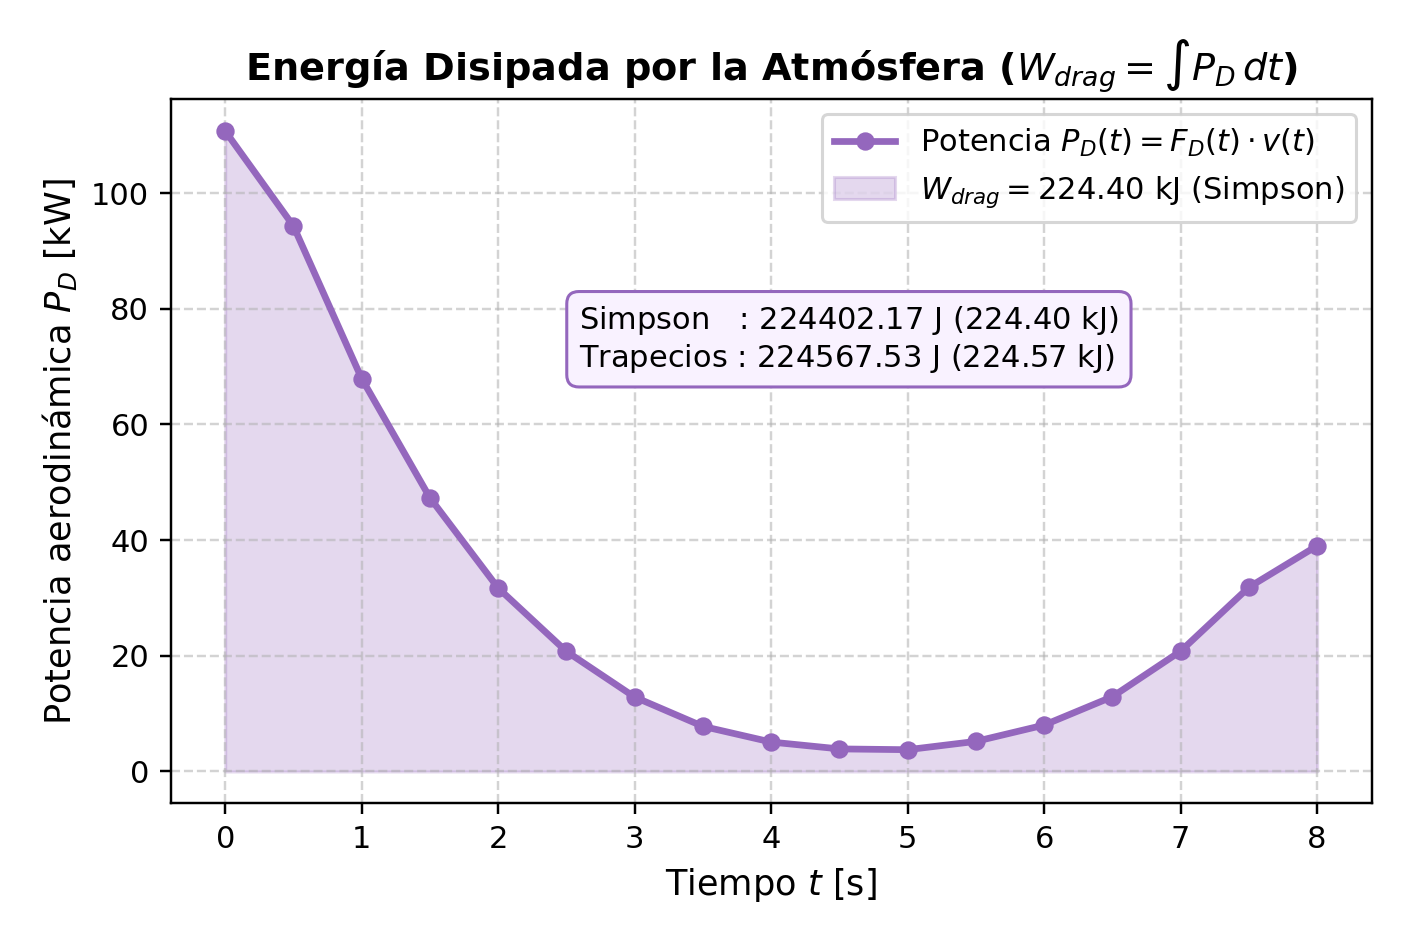
\includegraphics[width=\textwidth]{figures/fig_sec5.png}
        \end{column}
    \end{columns}
\end{frame}

% ============================================================================
% SLIDE 9: APARTADO 6 - BUSQUEDA DE RAICES
% ============================================================================
\begin{frame}{Apartado 6: Predicción de Impacto (Raíces No Lineales)}
    \begin{columns}[c]
        \begin{column}{0.43\textwidth}
            \textbf{Modelo de Caída ($t > 5\ \mathrm{s}$):}
            \[
                y(t) = 400 - 35(t-5) - 150\,e^{-0.2(t-5)} = 0
            \]
            \begin{itemize}
                \item \textbf{Justificación de $t_0$:} $y(8) \approx 212.7\ \mathrm{m} > 0$; la asíntota lineal cruza cero en $t \approx 16.43\ \mathrm{s} \Rightarrow t_0 = 15.0\ \mathrm{s}$, intervalo $[5.5, 50.0]\ \mathrm{s}$.
                \item \textbf{Newton-Raphson} (\texttt{tol=1e-10}): $15.948814\ \mathrm{s}$.
                \item \textbf{Bisección} (\texttt{tol=1e-10}): $15.948814\ \mathrm{s}$.
            \end{itemize}
        \end{column}
        \begin{column}{0.55\textwidth}
            \centering
            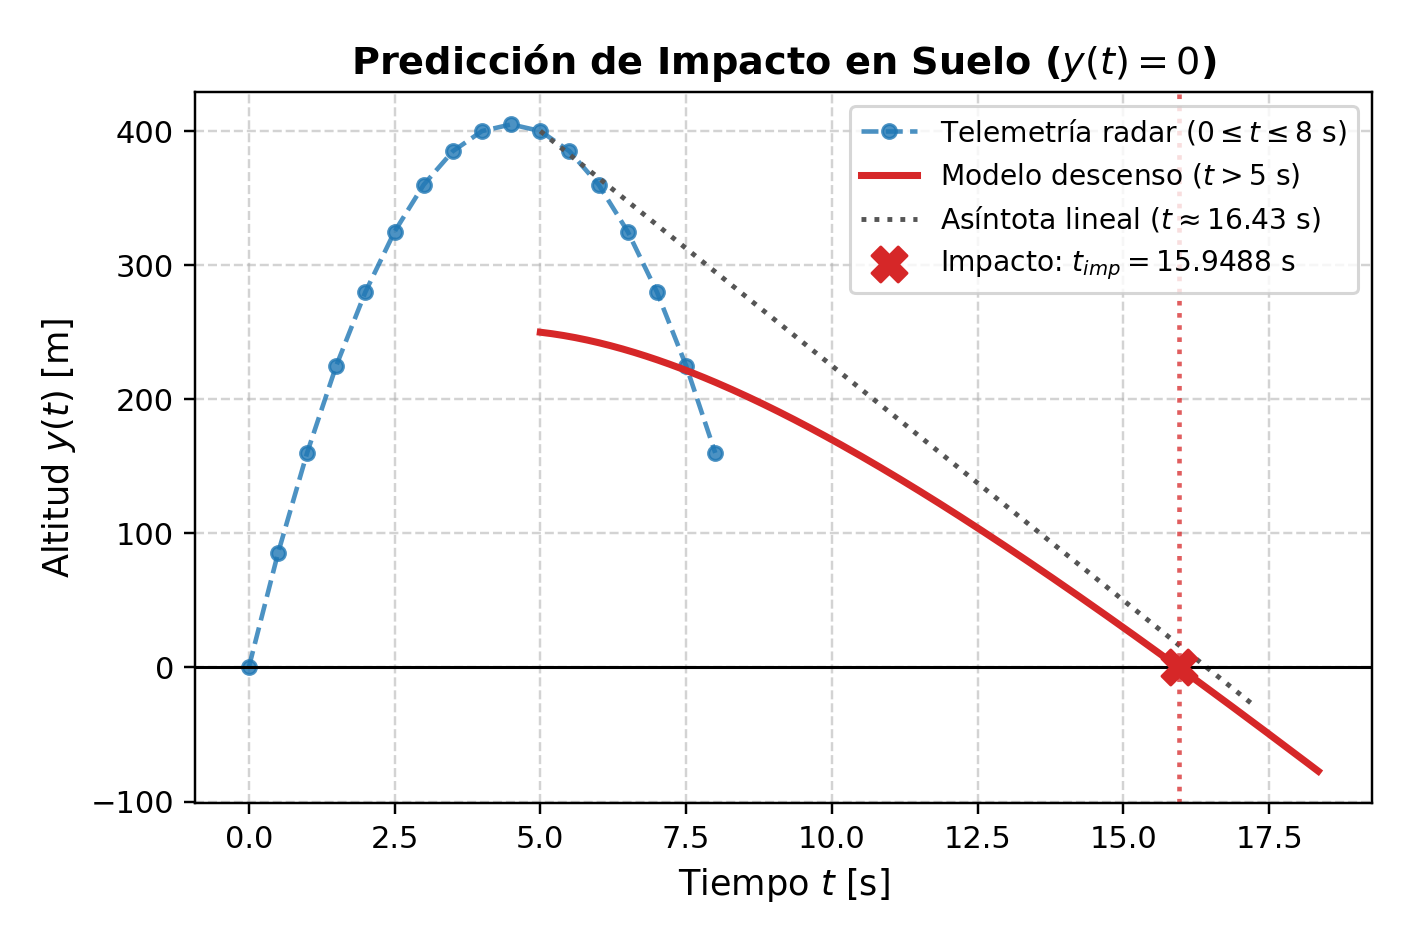
\includegraphics[width=\textwidth]{figures/fig_sec6.png}
        \end{column}
    \end{columns}
\end{frame}

% ============================================================================
% SLIDE 10: DASHBOARD INTERACTIVO EN MATPLOTLIB
% ============================================================================
\begin{frame}{Visualización: Dashboard Interactivo en Matplotlib}
    \begin{columns}[c]
        \begin{column}{0.36\textwidth}
            \textbf{Ventana única con \texttt{matplotlib.widgets}:}
            \vspace{0.15cm}
            \begin{itemize}
                \item \textbf{Navegación:} 6 botones (\texttt{Button}) para alternar vistas.
                \item \textbf{Sliders dinámicos:}
                \begin{itemize}
                    \item Altitud $h$ ($0$--$2500\ \mathrm{m}$) $\rightarrow$ Ap. 3 y 5.
                    \item Vel. caída $v_{\text{desc}}$ ($15$--$60\ \mathrm{m/s}$) $\rightarrow$ Ap. 6.
                \end{itemize}
                \item \textbf{Texto integrado:} Cajas \texttt{ax.text} con valores SI e interpretación.
                \item \textbf{Calidad científica:} Títulos, ejes con unidades, rejilla y leyendas.
            \end{itemize}
        \end{column}
        \begin{column}{0.62\textwidth}
            \centering
            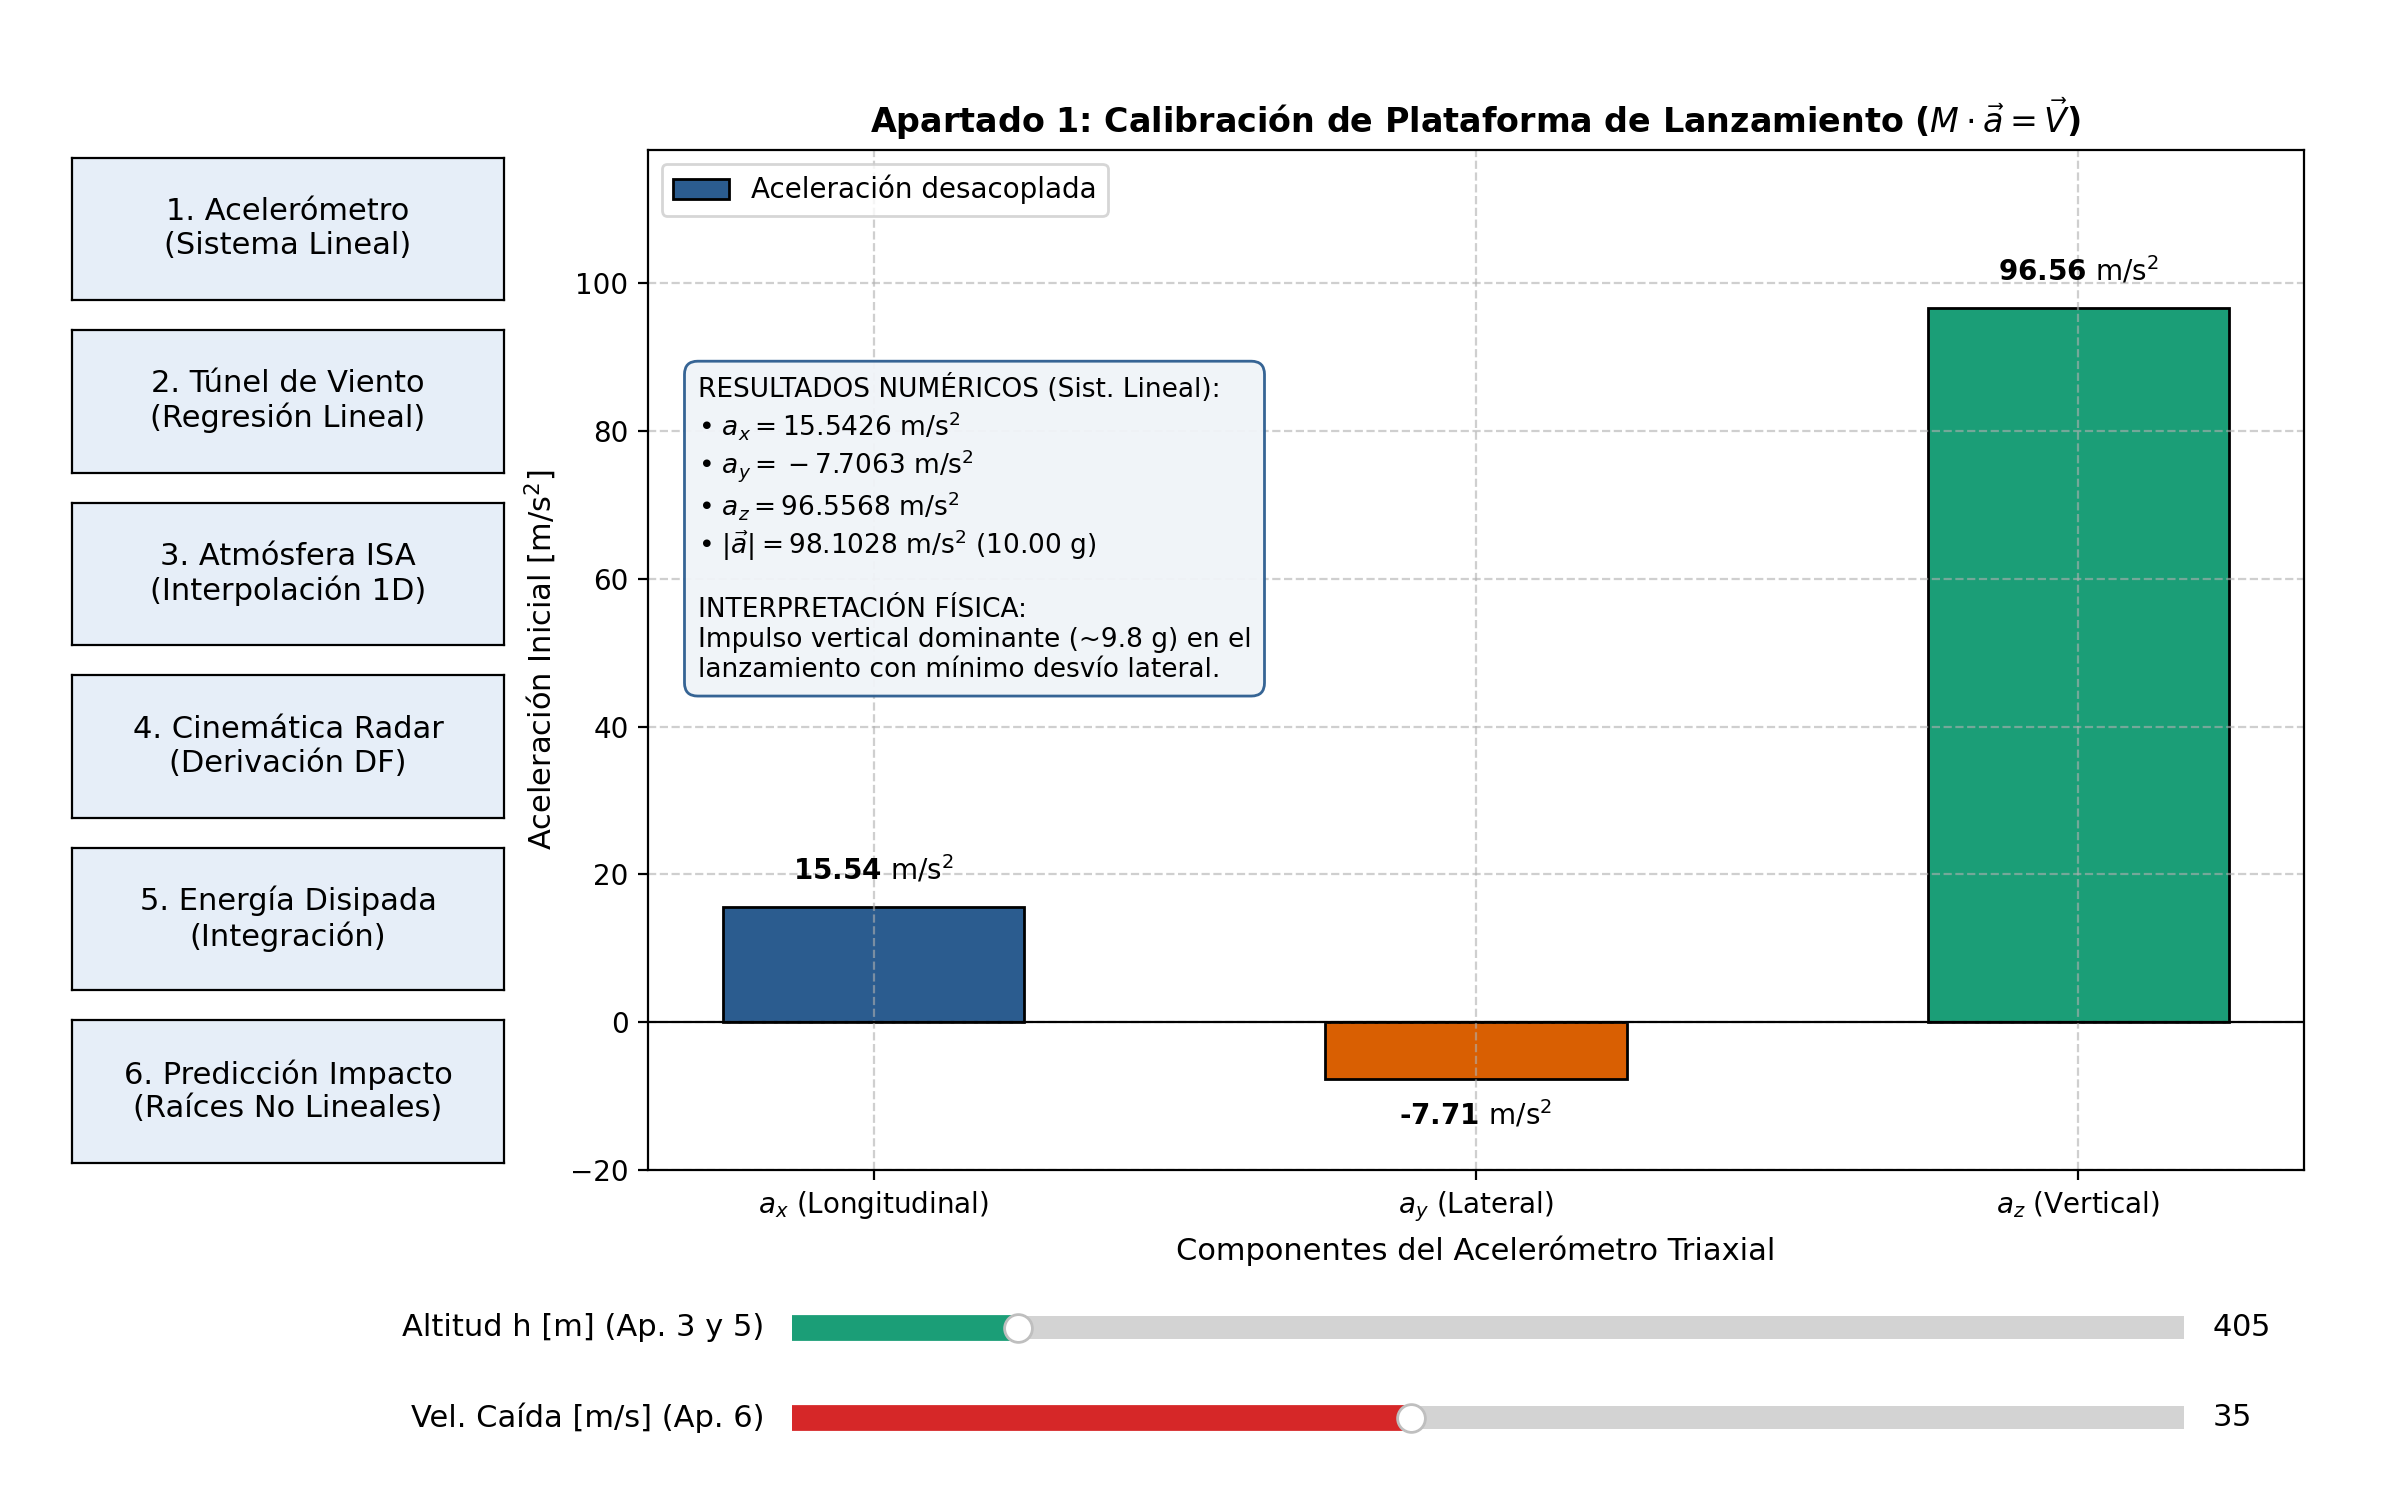
\includegraphics[width=\textwidth]{figures/fig_gui.png}
        \end{column}
    \end{columns}
\end{frame}

% ============================================================================
% SLIDE 11: VERIFICACION CON TESTS UNITARIOS FUNCIONALES
% ============================================================================
\begin{frame}[fragile]{Verificación con Tests Unitarios Funcionales}
    \begin{columns}[T]
        \begin{column}{0.48\textwidth}
            \begin{block}{\texttt{test\_math.py} (6/6 PASS)}
                Valida de forma aislada los métodos de \texttt{my\_math.py}:
                \begin{itemize}
                    \item Sistema lineal $2\times 2$ (\texttt{assert\_allclose}).
                    \item Regresión lineal exacta ($R^2 = 1.0$).
                    \item Interpolación cúbica exacta en $y=x^2$.
                    \item Derivada finita exacta en bordes e interior.
                    \item Simpson exacto en $y=3x^2$ y Trapecios.
                    \item Raíces de $x^2-4=0$ (Newton y Bisección).
                \end{itemize}
            \end{block}
        \end{column}
        \begin{column}{0.48\textwidth}
            \begin{block}{\texttt{test\_physics.py} (6/6 PASS)}
                Valida las invariantes físicas de \texttt{physics.py}:
                \begin{itemize}
                    \item Reconstrucción $M_{\text{calib}}\vec{a} = \vec{V}_{\text{medido}}$.
                    \item $(C_D A) \approx 0.025270\ \mathrm{m^2}$, $R^2 > 0.999$.
                    \item Acotación física $1.167 < \rho(405) < 1.225$.
                    \item Velocidad vertical nula en el apogeo ($v_y[9]=0$).
                    \item Consistencia Simpson vs. Trapecios ($<5\%$).
                    \item Residuo $|y(t_{\text{imp}})| < 10^{-8}\ \mathrm{m}$.
                \end{itemize}
            \end{block}
        \end{column}
    \end{columns}
    \vspace{0.25cm}
    \centering
    \small Ejecución verificada con Python 3.11: \textbf{12 / 12 tests superados} (paradigma funcional, sin clases).
\end{frame}

% ============================================================================
% SLIDE 12: SINTESIS DE RESULTADOS Y CONCLUSIONES
% ============================================================================
\begin{frame}{Síntesis de Resultados (SI) y Conclusiones}
    \centering
    \footnotesize
    \begin{tabular}{@{}llll@{}}
        \toprule
        \textbf{Apartado} & \textbf{Método Numérico} & \textbf{Resultado (SI)} & \textbf{Sentido Físico} \\
        \midrule
        1. Acelerómetro & Sistema lineal (LU) & $|\vec{a}| = 98.10\ \mathrm{m/s^2}$ & Impulso vertical $\approx 10.0\,g$ \\
        2. Túnel viento & Regresión lineal & $(C_D A) = 0.025270\ \mathrm{m^2}$ & Régimen subsónico ($R^2=0.9997$) \\
        3. Atmósfera ISA & Interpolación cúbica & $\rho(405\,\mathrm{m}) = 1.1777\ \mathrm{kg/m^3}$ & $-3.86\%$ respecto a nivel del mar \\
        4. Cinemática & Dif. finitas vector. & $v(0)=195.23\ \mathrm{m/s}$ & $v_y=0$ en apogeo ($t=4.5\ \mathrm{s}$) \\
        5. Energía drag & Simpson / Trapecios & $W_{\text{drag}} = 224.40\ \mathrm{kJ}$ & Disipación térmica atmosférica \\
        6. Impacto & Newton / Bisección & $t_{\text{imp}} = 15.9488\ \mathrm{s}$ & Convergencia idéntica ($t_0=15\ \mathrm{s}$) \\
        \bottomrule
    \end{tabular}

    \vspace{0.35cm}
    \begin{block}{Conclusiones}
        \begin{itemize}
            \item Arquitectura limpia y reutilizable: \texttt{my\_math.py} $\rightarrow$ \texttt{physics.py} $\rightarrow$ \texttt{gui.py} $\rightarrow$ \texttt{main.py}.
            \item Implementación vectorizada, validada físicamente en unidades SI y verificada con 12 tests funcionales.
        \end{itemize}
    \end{block}
\end{frame}

\end{document}
